\pdfoutput=1
% arXiv requires \pdfoutput=1 inside the first five lines to select pdfTeX.
% IEEEtran V1.8b (2015/08/26). Bundle IEEEtran.cls and main.bbl in the arXiv
% tarball: arXiv runs neither bibtex nor biber on an uploaded .bib file.
%
% No em dash or en dash appears in this document. In LaTeX source that means
% the triple-hyphen and double-hyphen ligatures are never used, including in
% bibliography page ranges, where a single hyphen is used instead.
\documentclass[conference]{IEEEtran}

\usepackage{etoolbox}
% IEEEtran.cls hardcodes a triple-hyphen ligature after "Abstract" and after
% "Index Terms", and IEEEtran.bst emits one for a repeated author and turns
% page ranges into the double-hyphen ligature. This project forbids both
% rendered dashes outright. The class file itself is NOT edited, because a
% modified IEEEtran.cls would be a format non-conformance a reviewer or an
% automated check would be right to flag. Instead the two class macros are
% patched in this preamble to use a colon, and the bibliography is
% post-processed by build.sh after bibtex runs. If either patch stops
% matching a future IEEEtran, the \PackageError below stops the build rather
% than letting a dash through silently.
\makeatletter
\patchcmd{\abstract}{---}{:\ }{}{\PackageError{titan}{abstract dash patch failed}{}}% dash-check-allow-this-line-removes-a-dash
\patchcmd{\IEEEkeywords}{---}{:\ }{}{\PackageError{titan}{keywords dash patch failed}{}}% dash-check-allow-this-line-removes-a-dash
\makeatother

\usepackage{graphicx}
\graphicspath{{../figures/}}
\usepackage{booktabs}
\usepackage{amsmath}
\usepackage{url}
\usepackage[hidelinks]{hyperref}

\begin{document}

\title{When a Full Barrier Beats a Store-Release, and When It Does Not:\\
A Pre-Registered Measurement Study of Ordering, Waiting and Arrival\\
Clustering in an SPSC Ring on a Fanless Apple M4}

\author{\IEEEauthorblockN{Nayan Pandit}
\IEEEauthorblockA{Indian Institute of Technology Patna, India\\
nayanpandit993281@gmail.com}}

\maketitle
\bstctlcite{bstctl:titan}

\begin{abstract}
The single-producer single-consumer ring is the hot path of a market-data feed
handler, and its loop body is small enough that the memory-ordering operation
is a large fraction of the work rather than a rounding error on it. We measure
that fraction on an Apple M4 and find it is 95.3 percent: the same ring with
all ordering removed runs at 10.185 cycles per message against 218.880 for an
acquire-release pair when the cursor line is contended. That unordered arm is
not a correct ring and is reported only as a cost floor. It failed its
checksum in all 180 of its epochs, while each of the four correct rings passed
in 180 of 180, so the 95.3 percent measures the distance to an unattainable
bound rather than to a usable alternative. Within that budget, the
choice of ordering construct behaves in a way no memory model describing this
hardware predicts. That a store-release can cost more than a stronger barrier
has been reported before, on other ARM parts and once on an Apple M1, in both
cases without a rule for when it happens; the rule is what we
measure. Replacing the release store, which LLVM emits as
\texttt{stlr} on the producer path and \texttt{stlur} on the consumer path,
with a \texttt{dmb ish} barrier followed by a plain store costs 2.5766 times
fewer cycles per message when the cursor line is contended, and 2.7008 times
more once the line is resident in L1, each at 30 of 30 independent launches. Both are cycle ratios
read from the hardware counters rather than nanosecond ratios, because a
registered check on the spread of core frequency across the arms failed and the
consequence of that failure was fixed before the run. Crossing the two halves of the acquire-release
pair over 30 independent launches localises the effect entirely to the store
side: substituting the release store alone accounts for a median 133.611 cycles of
the median 124.544 saved by substituting both, at 30 of 30 launches, while substituting the acquire load alone
saves 35.080, which is real at 30 of 30 but a quarter of the size and is paid
back when both are applied. The ranking of all four correct rings reverses
between the two caching configurations. A measurement hazard sits
underneath all of this, and it is not new. The core clock tracks how long a core
has been busy rather than how much work it was given, and Emurian et al.
\cite{emurian2014pitfalls} bound the resulting distortion at about 8 percent on
a server-class part, with up to 5.8 percent error on a nominal two times
speedup. On a fanless M4 the same hazard is 16.33 times, two orders of magnitude
larger, and it does not merely inflate a margin: the cheapest ordering at
200,000 messages is the dearest at 10,000,000, so run length decides which
construct a reader would choose. The power state of that run was not recorded, since the harness began
capturing it two days later, and on a fanless machine the power state bounds
the sustained clock. The arrival process moves the tail further than any ordering construct in this
paper does, and the statistic that captures it is not the one this work first
used. Holding the branching ratio of a Hawkes process at 0.8 fixes the Fano
factor of event counts near 25, while sweeping the kernel decay rate moves the
squared coefficient of variation of interarrival times from 1.1005 to 8.1921.
Across that ladder the Fano factor implies a ratio of 1.040 and the variability
term of Kingman's heavy-traffic approximation implies 7.444. The measured ratio
is 6.2317 at the median and 13.5030 at the quantile where the contrast peaks, in
30 of 30 launches, with 841 ns becoming 11356 ns at the same offered rate on the
same binary and the same messages. The periodic and Poisson references show no
effect against the low-variability arm, at 8 and 9 of 30. All results come from a pre-registered protocol, 87 hypothesis rows and five
exploratory calibrations, with thresholds fixed before each run, at least 20 independent launches per
comparison and 30 for all but the run-length sweep, within-launch pairing and
an exact two-sided sign test. Every figure regenerates from the
committed measurement files with one command; reproducing the measurements
themselves requires an Apple M4 on wall power.
\end{abstract}

\begin{IEEEkeywords}
memory consistency, Apple silicon, AArch64, lock-free queues, performance
measurement, measurement bias, hardware performance counters
\end{IEEEkeywords}

\section{Introduction}

A feed handler that reconstructs a limit order book from an exchange multicast
feed spends its time in a loop of a few instructions: read the producer's
cursor, read a slot, update book state, publish the consumer's cursor. The
cursors are shared between two cores, so each read and each publish carries a
memory-ordering obligation, and on a weakly ordered architecture that
obligation is discharged by a specific instruction chosen by the programmer
through a source-level annotation.

The prevailing guidance for such a loop is that the weak orderings are cheap
and should be preferred to sequential consistency, and that an explicit full
barrier is the expensive option of last resort. That guidance is sound as a
summary of the architecture manuals. It is also, on the machine measured here,
wrong about which of two correct rings is faster, wrong by a factor of 2.57,
and wrong in the opposite direction depending on whether a single cache line
happens to be resident.

The nearest prior work makes the gap explicit. Khayet and
Morrison~\cite{khayet2026arm} measure Apple M1 and M4 under Apple's
runtime-configurable total store order mode against native Arm mode across 49
application workloads, and conclude that the Arm memory model carries no
inherent performance advantage on Apple silicon, with typical execution times
within about 3 percent. They state that they leave the performance of atomic
read-modify-write operations and memory barriers to future work, on the stated
assumption that modern concurrent software is not bottlenecked on
synchronization. For the workloads they measure, that assumption is reasonable.
For the loop measured here it is false, and we measure the fraction rather than
asserting it: with ordering removed entirely the loop runs at 10.185 cycles per
message against 218.880 with an acquire-release pair, so 95.3 percent of the
contended loop is ordering. The unordered arm is a cost floor and not a correct
ring, and we report it as such: it failed its checksum in every one of its 180
epochs while each correct ring passed in 180 of 180. The fraction therefore
bounds what ordering costs, and does not name a cheaper ring that exists.

\subsection{Contributions}

\begin{itemize}
\item \textbf{The condition that governs the store-release anomaly.} That a
store-release can cost more than a stronger barrier is already
reported~\cite{liu2020barriers,arden2023riscv}, without a rule for when, and
Liu et al. recommend measuring it for that reason. The rule measured here is
caching state: substituting \texttt{dmb ish} and a plain store for the release
store costs 2.5766 times fewer cycles per message when the cursor line is
contended and 2.7008 times more when it is resident in L1, each at 30 of 30
launches, so the comparison changes sign rather than magnitude. Two runs with
different epoch counts agree on the contended figure to one part in a thousand.
The obvious explanation is excluded by the counters, within the scope the
counters actually cover: on the consuming thread, the barrier arm carries more
L1D load misses than the acquire-release arm in every configuration and is
faster when contended anyway. The qualifier is not decoration. Counting is per
thread on this unit, the measuring thread ran the consumer, and the two arms
differ in the instruction the producer executes, so this observation bounds the
consumer's load traffic and says nothing about the producer's.

\item \textbf{The effect is localised to the store side, by a pre-registered
cross of the two halves.} We measure four correct rings formed by crossing the
load side and the store side independently, so that each arm still carries
acquire semantics on every cursor read and release semantics on every publish,
whether from the instruction or from an adjacent barrier. The store-side share
of the total difference, taken as the median of the per-launch ratios rather
than as the ratio of the medians, which is 1.0728, is 1.0702 with a bootstrap
interval of [1.0621, 1.0866], at or above the pre-registered 0.70 in 30 of 30 launches; the
load-side share is 0.2797 and reaches that threshold in 0 of 30. The two
substitutions are strongly sub-additive, and adding the load-side barrier on
top of the store-side barrier costs 9.067 cycles.

\item \textbf{The ranking of all four correct rings reverses between caching
configurations.} Contended, the order is 85.269, 94.336, 183.800 and 218.880
cycles per message; L1-resident, it is 8.021, 8.053, 20.567 and 22.120. The
cheapest contended ring is the dearest resident one.

\item \textbf{A measurement hazard specific to heterogeneous consumer silicon.}
The core clock on this part tracks elapsed busy time rather than work
completed. A comparison that is stable in principle therefore moves by a stated
16.33 times between 200,000 and 10,000,000 messages, and the ordering that is
cheapest at the short run length is the dearest at the long one. This is a
post-2009 instance of the general phenomenon named by Mytkowicz et
al.~\cite{mytkowicz2009wrong}, whose demonstrated bias sources were UNIX
environment size and link order; duration-driven frequency scaling and
heterogeneous core residency did not exist on a general-purpose CPU at that
time.

\item \textbf{The lead results reproduce across time and a platform revision,
not merely across a re-analysis.} The barrier cross was re-run in full, 30
fresh launches three days after the original, on a macOS build the original
did not run on. The contended inversion returned at 2.5401 against a published
2.57, the resident one at 2.5146 against 2.75 with its sign intact, and both
caching rankings came back identical arm for arm. The arrival process result
was re-run the same way, 30 fresh launches two days later across the same
operating system update: the peak of the random over periodic curve returned
within 0.4 to 2.4 percent and the median within 0.7 percent of the original.
Both replications were registered with their tolerances before either ran, and
both retain every record, so each statistic above is recomputable from the
committed data rather than quoted from a summary.

\item \textbf{A protocol built so the conclusions survive the hazard.} Every
comparison here is pre-registered with pass and fail thresholds fixed before
the run, measured over independent process launches, 30 for every comparison
but the run-length sweep, which used 20 at each of its four message counts,
paired within each launch and tested with an exact two-sided sign test for
which 21 of 30 is the p < 0.05 threshold. Every figure regenerates from the committed
measurement files with one command.
\end{itemize}

\subsection{What this paper does not claim}

A third run settles which of those numbers to trust. The replication above was
measured in nanoseconds, because the hardware counters require root and an
unattended script must not carry a password prompt, and a nanosecond ratio is a
work ratio only if the two arms ran at similar clocks. Reading the counters
directly over 30 launches and 900 records gives 2.5766 contended and 2.7008
resident, each at 30 of 30. Recomputing the nanosecond ratios from the
committed records of the earlier run with the same aggregation puts the
contended figure 2.1 percent from its cycle counterpart and the resident figure
7.3 percent from its own, and the resident cycle figure within 1.8 percent of
the originally published 2.75. The frequency difference
between the two compared arms is 1.0086 contended and 1.0611 resident, which
accounts for the gap. The registered check on frequency spread was written over
all five arms rather than over the compared pair and failed at 1.1922, driven by
the unordered cost floor, which spends 10.198 cycles per message against 83.579
and does not hold the core at the same frequency. That specification fault is
recorded in the repository rather than repaired after the fact, and the
consequence registered before the run stands: the figures above are cycles.

The mechanism behind the store-side result is a hypothesis and is reported as
one. A release store must not become visible before prior accesses are
observable, and with a coherence miss in flight the measured cost is consistent
with the store stalling until that miss completes, where a barrier followed by
a plain store pays a fixed cost once and then retires into the store buffer.
That account would explain both the saving when the line is contended and the
penalty when it is not. It is not established here, and a queue-occupancy
explanation is not excluded: a barrier changes how far the producer runs ahead
of the consumer, and instrumenting ring occupancy inside the hot loop would
perturb the quantity being measured.

The results are from one Apple M4 in one fanless chassis, one ring, one padding
and one wait strategy, on performance cores. A cross-architecture control on
x86-64 is reported, and it is reported with the limitation that the host is
virtualized and exposes no frequency-scaling interface at all, so on that host
the absence of the run-length effect and the invisibility of the clock cannot
be told apart.

\section{Related Work}

\subsection{Measurement bias}

Mytkowicz et al.~\cite{mytkowicz2009wrong} established that measurement bias in
systems evaluation is both significant, in the sense that it can reverse a
conclusion, and commonplace. They demonstrated it from two sources, the size of
the UNIX environment and link order, and surveyed 133 papers from ASPLOS, PACT,
PLDI and CGO without finding one that adequately considered it.

The second result of this paper is an instance of that phenomenon rather than a
rediscovery of it, and the distinction is the bias source. The frequency a core
runs at on this part is a function of how long the core has been busy, not of
how much work it was given, so two implementations handed identical message
counts are measured at different clocks and the comparison between them moves
with run length. Neither that source nor heterogeneous core residency existed
on a general-purpose CPU in 2009. What is new is the specific source, its
measured size, and direct clock evidence for the mechanism.

\subsection{Total store order on Apple silicon}

Apple silicon implements a runtime-switchable total store order mode alongside
standard AArch64 weak ordering, used by the Rosetta 2 binary translator.
Wrenger et al.~\cite{wrenger2023tosting,wrenger2024m1} exploit that switch to
compare the two memory models with the rest of the machine held constant, and
report that total store order costs on average 8.94 percent on multi-threaded
SPEC CPU 2017 floating-point workloads on an M1.

That is a comparison of two hardware memory models with the program held fixed.
This paper compares ordering annotations and barrier placements within one
memory model with the hardware held fixed. The axes are orthogonal: a
whole-application figure for switching the machine's model does not predict a
2.57 times difference between two correct ways of writing the same ring under
the weak model.

\subsection{The store-release anomaly}

That a store-release can cost more than a semantically stronger barrier is not a
new observation, and this paper does not report it as one. Liu et
al.~\cite{liu2020barriers} measured ARM barriers across Kirin 960, Kirin 970,
Raspberry Pi 4 and Kunpeng 916. Their third observation states that the
store-release barrier does not always outperform stronger barriers. They report
it performing poorly on Kunpeng 916 and Raspberry Pi 4, including cross-node,
note that its overhead is unstable and sits between a full data synchronisation
barrier and a store-ordering data memory barrier, and say the phenomenon
recurred across several of their experiments. They offer no mechanism. They
state that no accurate public description of the instruction's implementation is
available, and they recommend comparing a store-release against a full barrier
before using one.

Arden et al.~\cite{arden2023riscv} met the same anomaly on Apple silicon while
proposing acquire and release instructions for RISC-V. Running a queueing
benchmark on an M1 with a compiler modified to emit bidirectional fences in
place of the weaker instructions, which raised the emitted barrier count by
roughly a factor of four and a half, they found that removing the weaker
instructions improved performance in some scenarios and called that result
unexpected. They attributed it to heavy data sharing between threads dominating
the cost, and described what remained as interference and noise.

Those two are the starting point here, not a finding. What neither supplies is a
condition. Liu et al. identify a platform and a placement rather than a rule,
and recommend measurement precisely because they have no rule to offer. Arden et
al. name data sharing and then set the residual aside. This paper supplies the
governing variable both were missing: whether the cursor line is contended or
resident in L1 decides the sign of the comparison, not merely its size. It does
so on a part neither of them measured, since the cores in their platforms are
Cortex-A53, A72 and A73 and none implements ARMv9; it localises the effect to
the store side by a pre-registered crossover rather than by inference; and it
checks the correctness of every arm instead of assuming it, which is how the
unordered arm was identified as a cost floor rather than an alternative.

\subsection{Pre-registration in empirical computer science}

Cockburn et al.~\cite{cockburn2020threats} surveyed a cross section of computer
science venues and concluded that a large proportion of the field faces the same
threats to replication as the disciplines already in open crisis, naming
performance analysis among the areas that validate claims by statistical
significance. Their recommendations include that the ACM encourage editors and
programme chairs to expect pre-registration of empirical studies, that authors
state whether a study was pre-registered, and that journals adapt review to
accept registered reports, which they call perhaps the most promising of all
the interventions they consider.

This study is conducted that way. Eighty-seven hypothesis rows and five exploratory
calibrations carry thresholds fixed before the corresponding measurement
existed, each registration was pushed to a public remote before the data it
governs was collected, and every verdict is recorded against the row that
predicted it, refutations included. Defects found during the work are published
in the repository rather than silently corrected, and they include the ones that
invalidated earlier claims of this paper's own. No pre-registered microbenchmark
study of memory ordering was located in the course of this work, and on the
evidence of that search the practice has not yet reached this part of the field.

\subsection{What queueing theory already predicts}
\label{sec:queueing}

The arrival process experiments in this paper measure a quantity that
classical queueing theory has an opinion about, and the paper would be
dishonest if it reported them as though it did not. Kingman's heavy traffic
analysis of the single server queue gives the mean waiting time as a product
of three factors: a utilisation factor $\rho/(1-\rho)$, a variability factor
formed from the squared coefficients of variation of the interarrival and
service time distributions, and the mean service time
\cite{kingman1961heavy,kingman1962queues}. A perfectly periodic arrival stream
has an interarrival coefficient of variation of zero and a Poisson stream has
one, so the periodic and Poisson arms of our experiment sit at two known
points on that variability axis. The direction of the effect we measure is
therefore not a discovery. What the formula does not supply, and what this
paper contributes, is the magnitude on a real software path, the shape of the
effect across the survival curve rather than at the mean, and the behaviour
under clustering.

The clustering result is where a careless reading of the approximation goes
wrong, and we went wrong there first. It is natural to characterise a
self-exciting arrival process \cite{hawkes1971spectra} by the Fano factor of
its event counts, which on our schedules rises from 0.9762 for the Poisson arm
to 25.5264 at a branching ratio of 0.9, and to conclude that such a process
must be far more expensive than Poisson at the same mean rate. The
variability term does not consume the Fano factor. It consumes the squared
coefficient of variation of the interarrival times, and on the identical
schedules that statistic moves only from 0.999926 to 1.024148 across the same arms.
The approximation therefore predicts almost no clustering penalty here, and
almost none is measured: indistinguishable from Poisson at roughly half of
the measured capacity, and 12 to 17 percent more expensive at the ceiling,
where the utilisation factor is large. Our measurement confirms the
approximation rather than contradicting it.

The contribution is the dissociation itself. Count-based and gap-based
descriptions of the same arrival process diverge by a factor of twenty-five
here, and only the gap-based one governs queueing. The Fano factor also
depends on the window used to compute it, moving from 6.0951 to 10.7775 on one arm
when only the sample length changed, while the coefficient of variation does
not. Practitioners in low-latency networking and in trading routinely
summarise burstiness by count statistics and infer a tail penalty from them.
On these schedules that inference fails, and the cause is that the
self-excitation timescale, the inverse of the kernel decay rate, is five
hundred times the mean interarrival gap, so clustering never reaches the
statistic that governs the queue.

Our Hawkes schedules are generated by Ogata's modified thinning algorithm
\cite{ogata1981thinning}, with the exponential kernel evaluated by an exact
recursion so that generation is linear rather than quadratic in the number of
events. The generator is validated against six analytic oracles and produces
bit identical schedules on Apple silicon and on x86 Linux.

\subsection{The deferred measurement}

Khayet and Morrison~\cite{khayet2026arm} extend that line to M1 and M4 with
microbenchmarks for load-load reordering, store-store reordering,
store-to-load forwarding and SIMD load throughput, and 49 application workloads
from SPEC CPU 2017, PARSEC, SPLASH-2x and OpenBenchmarking. Their statistical
practice is careful: at least eight runs per benchmark, continued until the 95
percent confidence interval falls within 1 percent of the median, with
randomized run order and non-parametric tests. Their conclusion is that the Arm
model has no inherent performance advantage on Apple silicon, that typical
execution times are within about 3 percent, and that the few severe cases are
attributable to Apple implementation artifacts rather than to the ordering
requirements of total store order.

Three relations to this work define its contribution.

First, they explicitly leave the performance of atomic read-modify-write
operations and memory barriers to future work; barriers appear in their study
only as experimental controls, and acquire, release and sequentially consistent
orderings are not measured. This paper measures exactly that, on one of the two
parts they used.

Second, the assumption under which that deferral is made, that modern
concurrent software is not bottlenecked on synchronization, holds for their
workloads and fails for this one. In SPEC and PARSEC the synchronization
operation is a small fraction of a large loop body; in a ring carrying market
data the loop body is a cursor load, a slot access, a cursor store and a
branch. We therefore test the premise rather than dispute the conclusion drawn
under it, and we measure the fraction rather than assert it.

Third, two methodological points, offered as complements. Their only
performance metric is execution time, which they state. On a part whose
performance and efficiency clusters run at fixed and very different clocks,
execution time and cycle count are not interchangeable: we measure a case in
which the efficiency cores take fewer cycles, between 0.808 and 0.984 of the
performance-core figure, and 3.057 times the wall time, so the two units order
the same pair of implementations oppositely. Separately, frequency scaling is
not discussed in their study, and a bias that is a function of run duration is
reproducible, so a protocol of repeating a run until its confidence interval is
tight does not by itself address it: repeating a short run faithfully
reproduces the short run's answer.

\section{Method}
\label{sec:method}

\subsection{Platform}

Every measurement reported as ours was taken on one machine, an Apple MacBook
Air identifying as Mac16,13 with an M4 and ten cores, four of them performance
cores, under macOS 27.2.1. Two operating system builds appear in the record,
26B123 and 26B131, because the system updated between two runs partway through
the work. The consequence was measured rather than assumed: the affected result
was replicated in full on the newer build, and every registered part of it
reproduced. The toolchain is a single \texttt{rustc} 1.92.0. The part is
fanless, which is not incidental: it is the reason run length changes a
comparison here and the reason the thermal state of a run is recorded with it.

Where a second platform appears it is labelled as such and used only as a
control. Those runs are on virtualised x86-64 hosts, for which no power state
exists; their results files say so in the field rather than leaving it blank.

\subsection{The ring under measurement}

The object of study is a single-producer single-consumer ring of 1024 slots,
with the producer and consumer cursors on separate 128-byte lines, which is the
coherence granule on this part rather than the 64 bytes an x86 port would use.
The loop body is a cursor load, a slot access, a cursor store and a branch, and
nothing else. That smallness is the point: it is what makes the ordering
operation a large fraction of the work rather than a rounding error on it, and
it is why the premise under which Khayet and Morrison defer barriers to future
work does not hold for this loop.

Five orderings are compared. An acquire load paired with a release store, the
same with a \texttt{dmb ish} barrier substituted on the load side alone, on the
store side alone, and on both, and an unordered arm with no ordering at all.
The instructions LLVM actually emits are recorded rather than assumed, by an
instruction census over the compiled library. The acquire-release arm compiles
to \texttt{ldapur} with \texttt{stlr} on the producer path and \texttt{ldapr}
with \texttt{stlur} on the consumer path, so both the scaled and the unscaled
RCpc forms appear and neither path uses \texttt{ldar}. Substituting the store
side replaces that release store with \texttt{dmb ish} followed by a plain
\texttt{str} on both paths, and adds exactly one barrier and one store to each
census. Naming a single instruction for the store side would have been wrong:
the two paths do not use the same one. The
unordered arm is a cost floor and not a candidate: it fails its checksum in
every epoch it runs, 0 of 180 passes, while each of the four correct rings
passes 180 of 180. Reporting it as an alternative would be reporting a ring that
does not work.

Each ordering is run in two caching states, with the cursor line contended
between cores and with it resident in L1, and under three waiting strategies, a
bare spin, a spin with \texttt{isb}, and \texttt{wfe} on a watched address. The
memory the ring uses is pinned before timing: the probe confirms 4096 of 4096
pages of a 64\,MiB region resident under \texttt{mlock}, with zero minor and
zero major faults taken during the hot write loop, on a part whose pages are
16384 bytes rather than 4096. The hot loop allocates nothing, which is measured
and not asserted: the probe runs it under a counting global allocator and
reports zero allocations.

\subsection{What this machine can and cannot resolve in time}

The timing facility advertises one resolution and delivers another, and a study
quoting nanoseconds on this part has to establish which.

\texttt{CNTFRQ\_EL0} reports 1000000000, so code that trusts the advertised
frequency computes a one nanosecond tick. The machine disagrees with itself:
\texttt{hw.tbfrequency} reports 24000000 and the Mach timebase is 125/3, which
is 41.667 nanoseconds. We settled it by measurement rather than by choosing a
source. Over ten million consecutive reads of the virtual counter, the value
advances by 42 units 1466253 times and by 41 units 731752 times, and 0.7558 of
consecutive pairs do not advance at all. A read costs about 10.20 nanoseconds,
and 34 pairs in ten million exceed eight steps.

So the usable grain is 41.667 nanoseconds behind a one gigahertz facade, three
reads in four return no change, and a single read costs a quarter of a tick.
Figure~\ref{fig:grain} shows the distribution. No claim about a single message
at tens of nanoseconds can rest on this counter, and none in this paper does.

\begin{figure}[t]
\centering
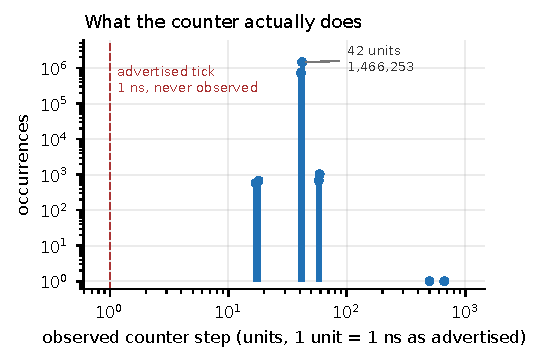
\includegraphics[width=\columnwidth]{fig-grain.pdf}
\caption{Ten million consecutive reads of the virtual counter on the M4. The
interface advertises a one nanosecond tick and the counter never once advances
by one. The mass sits at 41 and 42 units, which is the 24\,MHz hardware tick
that the Mach timebase of 125/3 implies, and 0.7558 of consecutive pairs do not
advance at all. A study quoting tens of nanoseconds from this counter is
quoting quantisation. Drawn from
\texttt{results/2026-11-21\_m4\_probe.txt}.}
\label{fig:grain}
\end{figure}

\subsection{Hardware counters, and the boundary we measured rather than assumed}

Cycle figures come from the Apple performance monitoring unit through the
\texttt{kperf} and \texttt{kperfdata} private frameworks, which are loaded by
\texttt{dlopen} because they do not exist as files on the filesystem. The event
database identifies itself as Apple silicon and carries 104 events, and all four
this work uses resolve against it: \texttt{FIXED\_CYCLES},
\texttt{FIXED\_INSTRUCTIONS}, \texttt{L1D\_CACHE\_MISS\_LD} and
\texttt{BRANCH\_MISPRED\_NONSPEC}. Counter reads are bracketed by \texttt{dmb
ish} and \texttt{isb sy} so that work inside the measured region cannot retire
outside it.

Counting is per thread, and the counters belong to whichever thread reads them.
In the runs reported here that thread ran the consumer loop, so every counter
figure in this paper describes the consuming side of the ring. We state this
because it is a real limit on what the counters can settle and because we did
not state it soon enough: a pre-registered threshold on retired store misses
was written against the consumer while the arms under test differ in the
producer's store instruction, and it returned zero on every arm of nine hundred
records. A diagnostic that drives three passes whose L1D behaviour is fixed in
advance confirms the event itself counts correctly under the same event set,
missing on close to every store over a buffer far larger than L1D and on
close to none over one that fits, so the zero was a correct measurement of the
wrong quantity. That threshold is recorded as unevaluable rather than passed, the
question is re-registered against a mode that keeps the producer on the
measuring thread, and the defect register carries the full account.

Three properties of the apparatus were measured, two of which bound what the
paper can claim.

First, accuracy. A dependent chain of exactly 102 instructions per iteration run
ten million times expects 1020000000 instructions. Twenty trials report between
1020167770 and 1020323076, an error between 0.0164 and 0.0317 percent, at 1.0007
to 1.0017 cycles per dependent add and 4.408 to 4.418 GHz. The counter is
trustworthy at the scale we use it.

Second, cost. A counter read has a median of 2557 cycles and 12675
instructions. Bracketing one message is therefore impossible by three orders of
magnitude, and every figure in this paper is accumulated over ten million
messages and divided. This is why the harness is built the way it is, and it is
a measured constraint rather than a stylistic choice.

Third, and least comfortable, the privilege boundary is not where the interface
says it is. The counting mode can be set to user only, and doing so makes no
difference. Over 100000 \texttt{getppid} calls, three trials per mode with the
modes alternated, the instruction count is 1110.2 per call under both modes, and
by the test's own logic a working user-only filter would leave a handful rather
than eleven hundred. We therefore state plainly that every counter figure in
this paper includes kernel work done on the thread's behalf, because that is
what the apparatus was measured to do. The residue in the accuracy check above,
about two hundred thousand instructions over twenty trials, is consistent with
it. The limitation is bounded: the hot loop makes no system call, and every
record carries its involuntary context switch count so a reader can see how much
kernel activity each measurement absorbed. Separately, \texttt{kpc\_cpu\_string}
returns empty on this part in both the unprivileged and the privileged pass,
while \texttt{kpc\_pmu\_version} is 0 unprivileged and 2 under root, so one of
those two is privilege-gated and the other is simply empty here.

\subsection{The independent launch as the unit of observation}

A single process launch is one observation. Within a launch, every arm under
comparison runs in that same process, so a pair is formed inside one launch and
never across two. This is what makes the comparison robust to anything that
varies between launches, including the frequency the core happens to settle at,
the placement the scheduler chooses, and the thermal state the machine starts
in. It is also what forced the decay-rate ladder to be added as a parameter
rather than run as separate processes: several arrival kernels have to exist
inside one launch for the pairing to hold.

Unless a row states otherwise, a comparison runs 30 launches of three epochs
each at ten million messages. The run-length sweep uses 20 launches at each of
its four message counts, which the abstract states rather than averaging over.
Verdicts use the exact two-sided sign test on the per-launch direction, for
which 21 of 30 is the threshold at $p < 0.05$. We report the count and the exact
$p$ value, never a normal approximation, and we report the direction and the
magnitude as separate questions, because only the direction distinguishes
competing accounts in the arrival experiments.

\subsection{Tail estimation}

Latency distributions are summarised by a complementary cumulative distribution
over 65 logarithmically spaced tail quantiles, recorded per arm, per wait, per
epoch and per launch. Quantiles supported by fewer than ten observations are
gated out rather than reported, so a tail figure is never read off a handful of
samples. Where two arms are contrasted, the ratio is formed quantile by quantile
within a launch and the comparison is taken at the quantile where the ratio is
largest, with that quantile reported alongside the ratio. Reporting a single
tail percentile would hide where on the curve an effect lives, and in this work
the location moves between arms.

\subsection{Thermal and power state}

Every run that measures time on the M4 is taken on wall power, and the delivery
script refuses to start otherwise. The power state is read at the start and at
the end of each run and recorded in the results file. Files that predate the
introduction of that field say so explicitly, and the two virtualised x86-64
controls and the pure-computation calibration record that the field does not
apply to them with the reason. No file is silent on it, which a gate enforces.

Because \texttt{powermetrics} and Instruments take exclusive ownership of the
performance monitoring unit, a counter run checks that neither is active before
it begins rather than failing obscurely partway through.

\subsection{Pre-registration, and the gates that enforce it}

Each hypothesis is a row carrying its thresholds, written and committed before
the measurement it governs exists, and pushed to a public remote before the data
is collected, so the ordering is externally checkable rather than asserted. The
verdict is recorded against the row that predicted it, including every
refutation. Where a threshold failed, the registered consequence was followed
rather than reinterpreted: the first three contributions of this paper are
reported in cycles rather than nanoseconds for exactly that reason.

Seven automated checks run on every change. They verify that no dash reaches the
rendered document, that every number the manuscript asserts is either present in
a results file or declared as derived, quoted or typeset with its source, that
no line in a results file wears a record prefix without carrying data, that
every number on every figure reproduces from an independent recomputation with
its own parser and its own statistics, that a set of semantic invariants hold
between the manuscript and the registration table, and that every results file
states its power condition. The checks that matter most are the semantic ones,
because the mechanical ones passed for days while the paper compared the wrong
statistic.

Defects found during the work are published in the repository rather than
silently corrected. Sixteen are recorded at the time of writing, and they
include the ones that invalidated earlier claims of this paper, the one where a
registered threshold was specified over the wrong set of arms, and the one where
a validation returned a negative answer that nobody read.

\subsection{Artifact}

The repository carries 323001 committed records across 38 results files, the
registration table, the defect register, the analysis scripts and the manuscript
source. Each figure regenerates from committed data by a script that shares no
code with the one that produced the numbers it checks. Nothing in the paper is
computed at build time from a fresh measurement, so building the document cannot
change a reported figure.

\bibliographystyle{IEEEtran}
\bibliography{refs}

\end{document}
